\chapter{Стегоанализ}
\section{Методы стегоанализа}
Основными методами, применяемыми в стегоанализе, являются визуальные методы и статистические методы.

Субъективная атака проста по своей сути: аналитик пытается ``на глаз'' определить, содержит ли контейнер стего.
Однако эта атака может применяться в различных вариациях. Например, анализу может подвергаться не само изображение,
а какой-то его канал, или же изображение, полученное из данного отбрасыванием нескольких старших бит.

Статистические методы основаны на использовании различных статистик изображения и том факте,
что эти статистики могут различаться для пустого и заполненного стегоконтейнера.

\section{Субъективная атака LSB}
Метод LSB является легко обнаружимым.
Для начала рассмотрим самую простую ситуацию: допустим,
что сообщение, скрытое в стего, не зашифровано.
В таком случае стегоконтейнер поддается визуальной атаке,
а именно: попробуем посмотреть на визуальное представление
последнего бита сообщения. Для этого используем код,
представленный в листинге~\ref{code:visual-lsb}.
\lstinputlisting[language=Python, label={code:visual-lsb}, style=simplecode, caption=Визуализация LSB, frame=single]{Code/visual_lsb.py}
Полученные изображения можно увидеть на рисунке~\ref{img:bw-lsb}.
Как видно, наименее значащий бит оригинального изображения распределен
шумоподобно, в то время как у стегоконтейнера этот бит
вносит в изображение какую-то струкуру. Так происходит из-за
неравномерного распределения символов в исходном сообщении.
Также из изображения можно увидеть примерную длину сообщения.
\begin{figure}[ht!]
    \centering
    \begin{subfigure}{.5\textwidth}
      \centering
      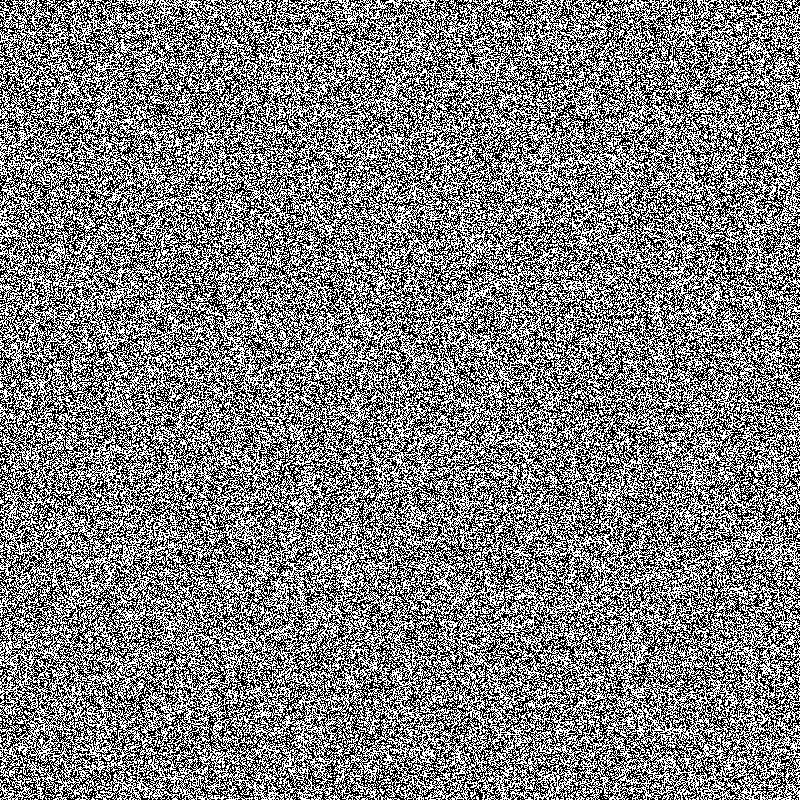
\includegraphics[width=.9\linewidth]{PNG/BW_Lenna.png}
      \caption{Оригинал}
      \label{img:bw-lenna-png}
    \end{subfigure}%
    \begin{subfigure}{.5\textwidth}
      \centering
      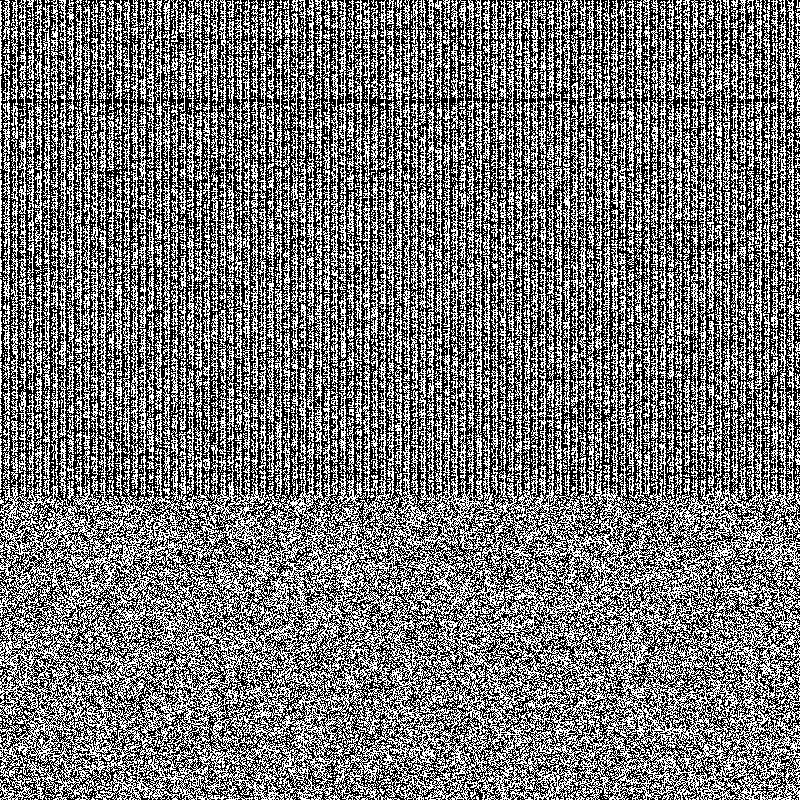
\includegraphics[width=.9\linewidth]{PNG/BW_LSB_Lenna.png}
      \caption{После применения LSB}
      \label{img:bw-lenna-lsb}
    \end{subfigure}
    \caption{Наименее значащий бит до и после LSB}
    \label{img:bw-lsb}
\end{figure}

\section{Атака оценки числа переходов значений младших бит в соседних элементах контейнера}
Допустим, что стегосообщение предварительно было зашифровано и сокрыто методом LSB.
В таком случае сообщение внутри контейнера будет обладать предельной энтропией,
а это значит, что наименее значимый бит контейнера будет распределен равномерно:
50\% объема будет занимать 0 и другие 50\% будет занимать 1. При этом два соседних
наименее значимых бита не будут скоррелированы. Однако в реальных изображениях это не так.
В реальном изображении соседние пиксели скоррелированы, и ненулевая вероятность того,
что они окажутся одинаковыми. Несмотря на то, что изображение~\ref{img:bw-lenna-png}
выглядит как шум, в нем есть некоторая статистическая структура. Чтобы выявить ее,
нужно попарно сравнить 2 соседних пикселя и посчитать, какой процент этих пикселей совпал.
Такое сравнение проводит в листинге~\ref{code:lsb-correlation}.
\lstinputlisting[language=Python, label={code:lsb-correlation}, style=simplecode, caption=Корреляция LSB, frame=single]{Code/lsb_correlation.py}
Вывод программы следующий: ``Original: P(False) = 0.46, P(True) = 0.54; Stego: P(False) = 0.5, P(True) = 0.5''.
Как видно, у оригинального сообщения совпадение и несовпадение двух соседних наименее значимых битов не равновероятны. 

\section{Атака хи-квадрат}
Допустим, что мы оказались в похожей ситуации: зашифрованное сообщение
было сокрыто методом LSB, --- но в этот раз в контейнере соседние элементы не скоррелированы.
Построим гистаграмму элементов контейнера и рассмотрим элементы, отличающиеся друг от друга в младшем бите.
Если это незаполненный стегоконтейнер, то частота двух соседних элементов $a$ и $b$ может сильно отличаться.
Однако если к такому контейнеру применить LSB, то в паре двух соседних значений $a$ в 50\%
случаев не изменится, и в 50\% случаев изменится на единицу. То же самое произойдет и с $b$.
Допустим, что $a$ был четным. Тогда в новом распределении частота $a$ будет равна $\dfrac{ f(a) + f(b)}{2}$,
где $f$ -- функция распределения частот в незаполненном контейнере. То же самое касается и $b$.
То есть соседние элементы будут распределены одинаково. На этом и основана атака хи-квадрат.

Критерий согласия Пирсона (критерий согласия $\chi^2$) --- это критерий принадлежности наблюдаемой
выборки $x_1, x_2, \dots , x_3$ теоретическому закону распределения $F(x, \theta)$,
где $\theta$ --- это известный параметр распределения.
Процедура проверки гипотез с использованием критерия$\chi^2$ предусматривает группирование наблюдений.
Область определения случайной величины разбивают на $k$
непересекающихся интервалов граничными точками
$x_{(0)}, x_{(1)}, \dots, x_{(k)}$.
В соответствии с заданным разбиением подсчитывают число $n_i$ выборочных значений,
попавших в i-й интервал, и вероятности попадания в интервал
$P_i(\theta) = F(x_{(i)}, \theta) - F(x_{(i - 1)}, \theta))$
соответствующие теоретическому закону с функцией распределения $F(x, \theta)$.
При этом $n = \sum_{i = 1}^{k} n_i$ и $\sum_{i = 1}^{k} P_i(\theta) = 1$.
В основе критерия согласия Пирсона лежит измерение отклонений
$\dfrac{n_i}{n}$ от $P_i(\theta)$.
Статистика критерия согласия $\chi^2$ Пирсона определяется соотношением~\ref{eq:chi-2}.
\begin{equation}
    \label{eq:chi-2}
    \chi^2 = n \sum_{i=1}^k \dfrac{(n_i / n - P_i(\theta))^2}{P_i(\theta)}
\end{equation}

Выделим из изображения все пары элементов, которые отличаются только в младшем бите.
Обозначим такие пары через $(2m, 2m + 1)$. Пусть $h_i$ обозначает гистограмму наблюдаемого
распределения элементов.
Введем новое наблюдаемое распределение $\{o_m\}$ равное $o_m = h_{2m}$
и теоретическое распределение $\{e_m\}$ равное $e_m = \dfrac{h_{2m} + h_{2m + 1}}{2}$.
Разница между этими двумя распределениями измеряется критерием~\ref{eq:chi-stego}
с $(\nu - 1)$ степенями свободы, где $\nu$ --- количество пар, отличающихся в младшем бите.
\begin{equation}
    \label{eq:chi-stego}
    \chi^2 = \sum_{e_m \neq 0} \dfrac{(o_m - e_m) ^ 2}{e_m}
\end{equation}

Степень сходства двух распределений $\{o_m\}$ и $\{e_m\}$ после этого считается
с помощью функции распределения по формуле~\ref{eq:chi-cdf}.
\begin{equation}
    \label{eq:chi-cdf}
    p = 1 - \int_{0}^{\chi^2} \dfrac{t^{(\nu - 2)/2}e^{-t/2}}{2^\nu\Gamma(\nu/2)}dt
\end{equation}

Реализация атаки на python представлена в листинге~\ref{code:chi}.
\lstinputlisting[language=Python, label={code:chi}, style=simplecode, caption=Атака хи-квадрат, frame=single]{Code/chi.py}
Программа выводит 0.0 для пустого контейнера и 0.99 для заполненного.

\section{Методы противодействия}
Для эффективного противодействия описанным статистическим и субъективным
атакам следует пользоваться следующими рекомендациями при построении
стеганографического алгоритма:
\begin{enumerate}
    \item Сообщение должно встраиваться в зашифрованном виде для предотвращения
    субъективных и иных атак.
    \item Сообщение должно встраиваться не в подряд идущие элементы контейнера,
    а в случайно выбранные элементы, например, с использованием генератора псевдослучайных
    чисел.
    \item Сообщение должно заполнять лишь малую часть емкости контейнера. Иначе
    оно может нарушить статистическую структуру контейнера. Так, например,
    атака хи-квадрат работает намного хуже, когда сообщение рассеяно по всей длине контейнера.
\end{enumerate}